\documentclass[a4paper, 12pt]{ltjsarticle}

\usepackage{luatexja}
\usepackage{amsmath, amssymb} % 数学?
\usepackage{ascmac} % 枠付き文書
\usepackage{bm} % 斜線太字ベクトル?
\usepackage{comment} % 複数行のコメントアウト
\usepackage{color} % よく分からん
\usepackage{graphicx} % 画像の挿入
\usepackage{listings, jvlisting} % ソースコードの挿入
\usepackage{url}

\lstset { % パッケージの追加設定
  frame={single},
  basicstyle={\small\ttfamily},
  tabsize=4
}

\begin{document} % 本体?ここから

\title{
  report sample with Lua{\LaTeX}
}
\author{
  hoge hige
}
\date{\today}
\maketitle % タイトルここまで

\tableofcontents % 目次
\newpage

\section{はじめに}
これは,大学のレポート課題用のテンプレートレポジトリです.


\section{引用てすと}
\subsection{サンプル}
引用\cite{hoge}だよーん


\section{数式テスト}
TeX clipというサイトのテンプレをパクった.

TeX clipはパワポにコピペする時に便利ですね

ちなみに,\verb | align,gather,...などがあり,*を付けると式の番号が付かない |

\begin{gather}
  \left( \int_0^\infty \frac{\sin x}{\sqrt{x}} dx \right)^2 =
  \sum_{k=0}^\infty \frac{(2k)!}{2^{2k}(k!)^2} \frac{1}{2k+1} =
  \prod_{k=1}^\infty \frac{4k^2}{4k^2 - 1} = \frac{\pi}{2}
\end{gather}


\section{画像の埋め込み}
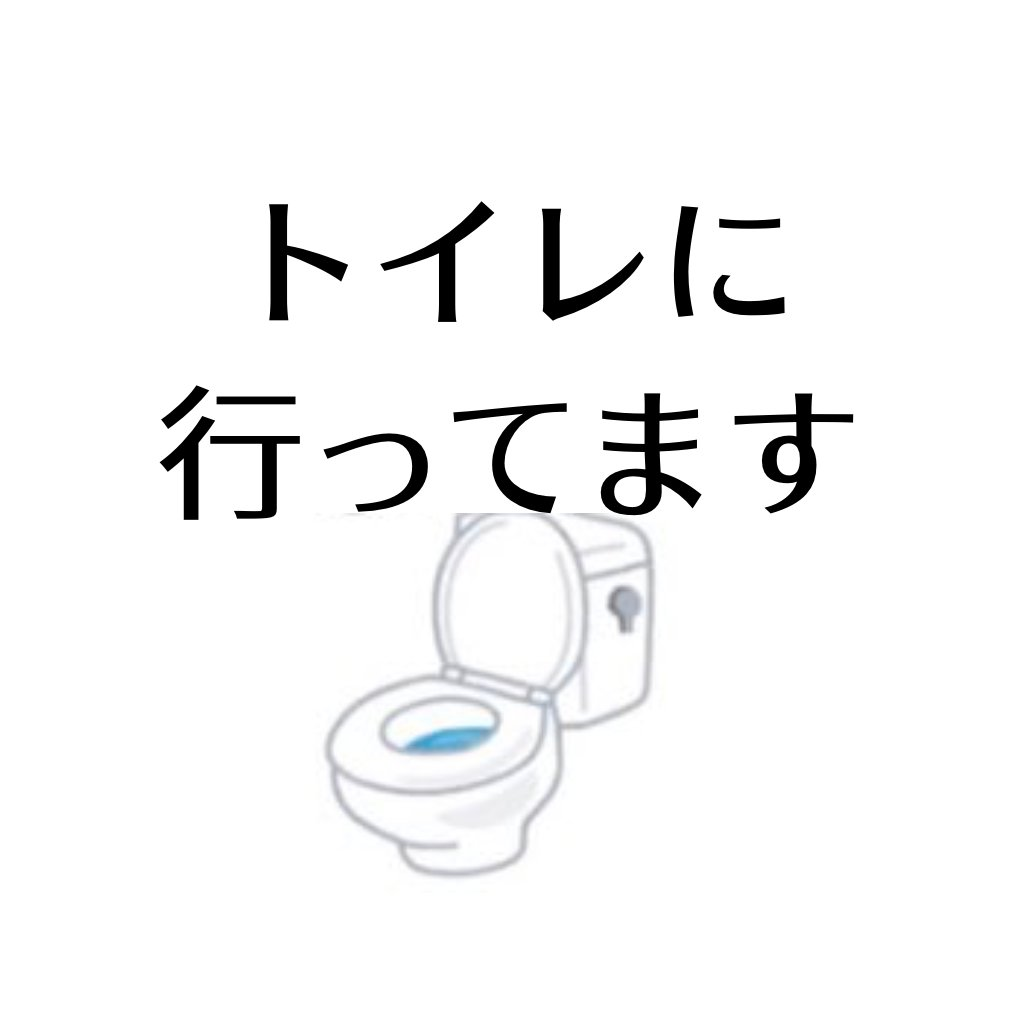
\includegraphics[scale=0.5]{./image.jpg}

% \begin{figure}[h]
%   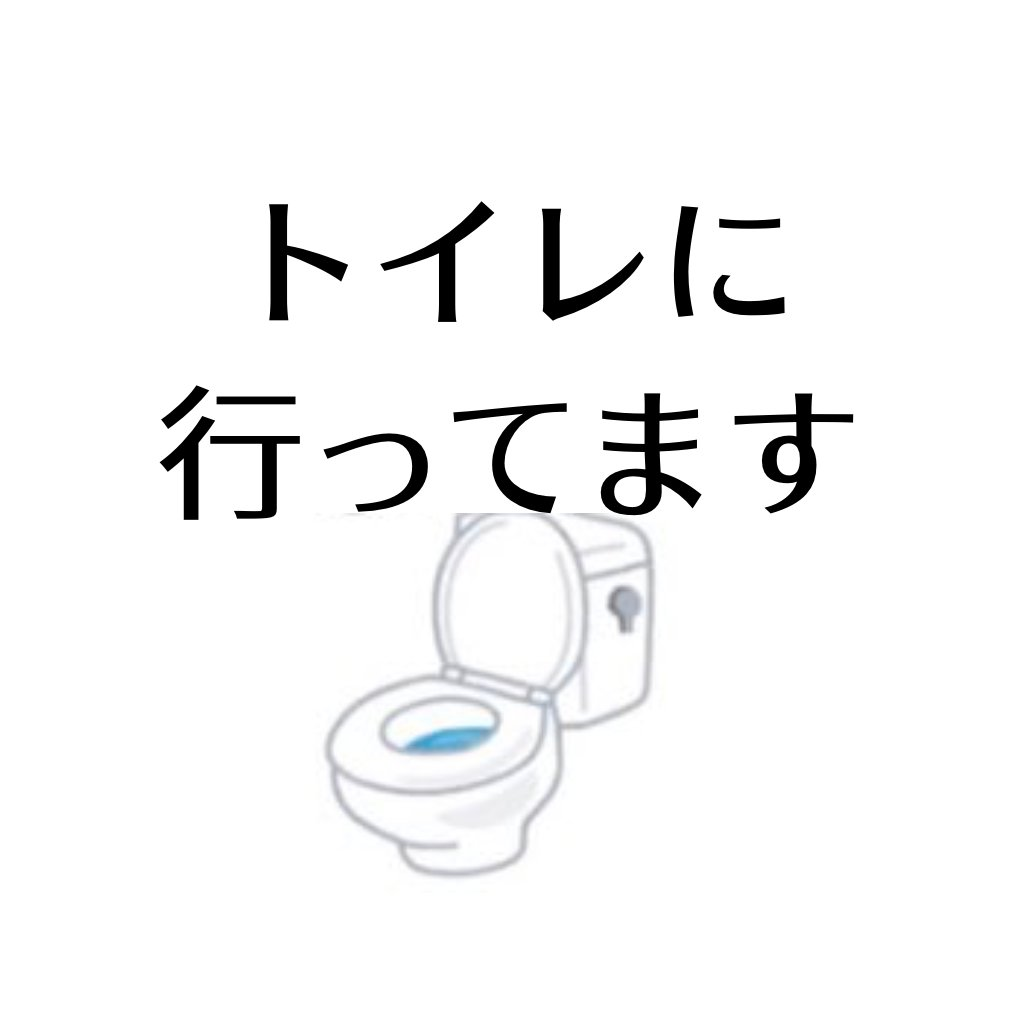
\includegraphics[scale=0.5]{./image.jpg}
%   \caption{write description here}
% \end{figure}


\section{他のTexファイル読み込みてすと}
\verb | % !TEX root = main.tex

\section{さぶファイルてすと}
これは,sub.texの内容です.
 でページ内に埋め込み |
\verb | \include{hoge.tex}で前後を改ページして埋め込み|

埋め込みたいファイル(sub.tex)の先頭に
\verb | % !TEX root = main.tex |
と書くのを忘れない

% !TEX root = main.tex

\section{さぶファイルてすと}
これは,sub.texの内容です.



\section{コードの挿入}

Flaskのサンプルコードを以下に示す

\begin{lstlisting}[caption=main.py]
from flask import Flask

app = Flask(__name__)
app.route("/")
def index():
  return "hello world with flask"

if __name__ == "__main__":
  app.run()
\end{lstlisting}


\section{箇条書き}

HTMLと同じ感じで
\\ ul(UnOrderedList)
\\ ol(OrderedList)
をスニペット登録している

\begin{itemize}
  \item 点の箇条書き
  \item 点の箇条書き
  \item 点の箇条書き
  \item 点の箇条書き
\end{itemize}

\begin{enumerate}
  \item 数字の箇条書き
  \item 数字の箇条書き
  \item 数字の箇条書き
  \item 数字の箇条書き
  \item 数字の箇条書き
  \item 数字の箇条書き
\end{enumerate}


\section{枠付き文章}

tbox: Text BOX

ttbox: Title Text BOX

\begin{screen}
  tboxスニペットで,角丸枠付き文章
  tboxスニペットで,角丸枠付き文章
  tboxスニペットで,角丸枠付き文章
  tboxスニペットで,角丸枠付き文章
  tboxスニペットで,角丸枠付き文章
  tboxスニペットで,角丸枠付き文章
  tboxスニペットで,角丸枠付き文章
  tboxスニペットで,角丸枠付き文章
\end{screen}

\begin{itembox}{タイトルだよ}
  ttboxスニペットで,タイトル付き,角丸枠付き文章
  ttboxスニペットで,タイトル付き,角丸枠付き文章
  ttboxスニペットで,タイトル付き,角丸枠付き文章
  ttboxスニペットで,タイトル付き,角丸枠付き文章
  ttboxスニペットで,タイトル付き,角丸枠付き文章
  ttboxスニペットで,タイトル付き,角丸枠付き文章
  ttboxスニペットで,タイトル付き,角丸枠付き文章
\end{itembox}


\section{おわりに}
LuaLaTeX + vscode + bibの情報が全然無くてとても大変だった

\bibliographystyle{junsrt}
\bibliography{references}

\end{document}
